\documentclass[a4paper]{article}

\newcommand{\worktype}{Лабораторная работа №1}
\newcommand{\workname}{Разработка программы для ПЛК в системе Codesys 3.5}
\newcommand{\studentname}{Овчинников П.А.}
\newcommand{\teachername}{Крылова А.А.}
\newcommand{\varnum}{6}
\newcommand{\copyrightyear}{2025}

\input{~/Документы/latex-boilerplates/settings.tex}

% \showTOCtrue

\begin{document}
\documentclass[a4paper]{article}

\newcommand{\worktype}{Домашняя работа №3}
\newcommand{\workname}{Плоский изгиб балки}
\newcommand{\teachername}{Моторин А.С.}
\newcommand{\studentname}{Овчинников П.А.}
\newcommand{\varnum}{10}
\newcommand{\groupnumber}{R3341}

\input{~/Documents/latex-boilerplates/settings.tex}

\begin{document}
\documentclass[a4paper]{article}

\newcommand{\worktype}{Домашняя работа №3}
\newcommand{\workname}{Плоский изгиб балки}
\newcommand{\teachername}{Моторин А.С.}
\newcommand{\studentname}{Овчинников П.А.}
\newcommand{\varnum}{10}
\newcommand{\groupnumber}{R3341}

\input{~/Documents/latex-boilerplates/settings.tex}

\begin{document}
\documentclass[a4paper]{article}

\newcommand{\worktype}{Домашняя работа №3}
\newcommand{\workname}{Плоский изгиб балки}
\newcommand{\teachername}{Моторин А.С.}
\newcommand{\studentname}{Овчинников П.А.}
\newcommand{\varnum}{10}
\newcommand{\groupnumber}{R3341}

\input{~/Documents/latex-boilerplates/settings.tex}

\begin{document}
\input{~/Documents/latex-boilerplates/titlepage.tex}

\end{document}

\end{document}

\end{document}

\addsection{Задание}
\textbf{Автоматизация системы осушения подвала.} При срабатывании верхнего порогового датчика уровня включается насос, загорается желтая лампа. При срабатывании нижнего датчика уровня насос выключается, гаснет желтая лампа и зажигается зелёная.\\[0.5em]
Входы:
\begin{itemize}
    \item Пороговый датчик уровня жидкости верхний \verb|(булево значение)|
    \item Пороговый датчик уровня жидкости нижний \verb|(булево значение)|
\end{itemize}

Выходы:
\begin{itemize}
    \item Реле, включающее насос \verb|(булево значение)|
    \item Желтая лампа \verb|(булево значение)|
    \item Зеленая лампа \verb|(булево значение)|
\end{itemize}

\addsection{Структурная схема}
\begin{figure}[H]
    \centering
    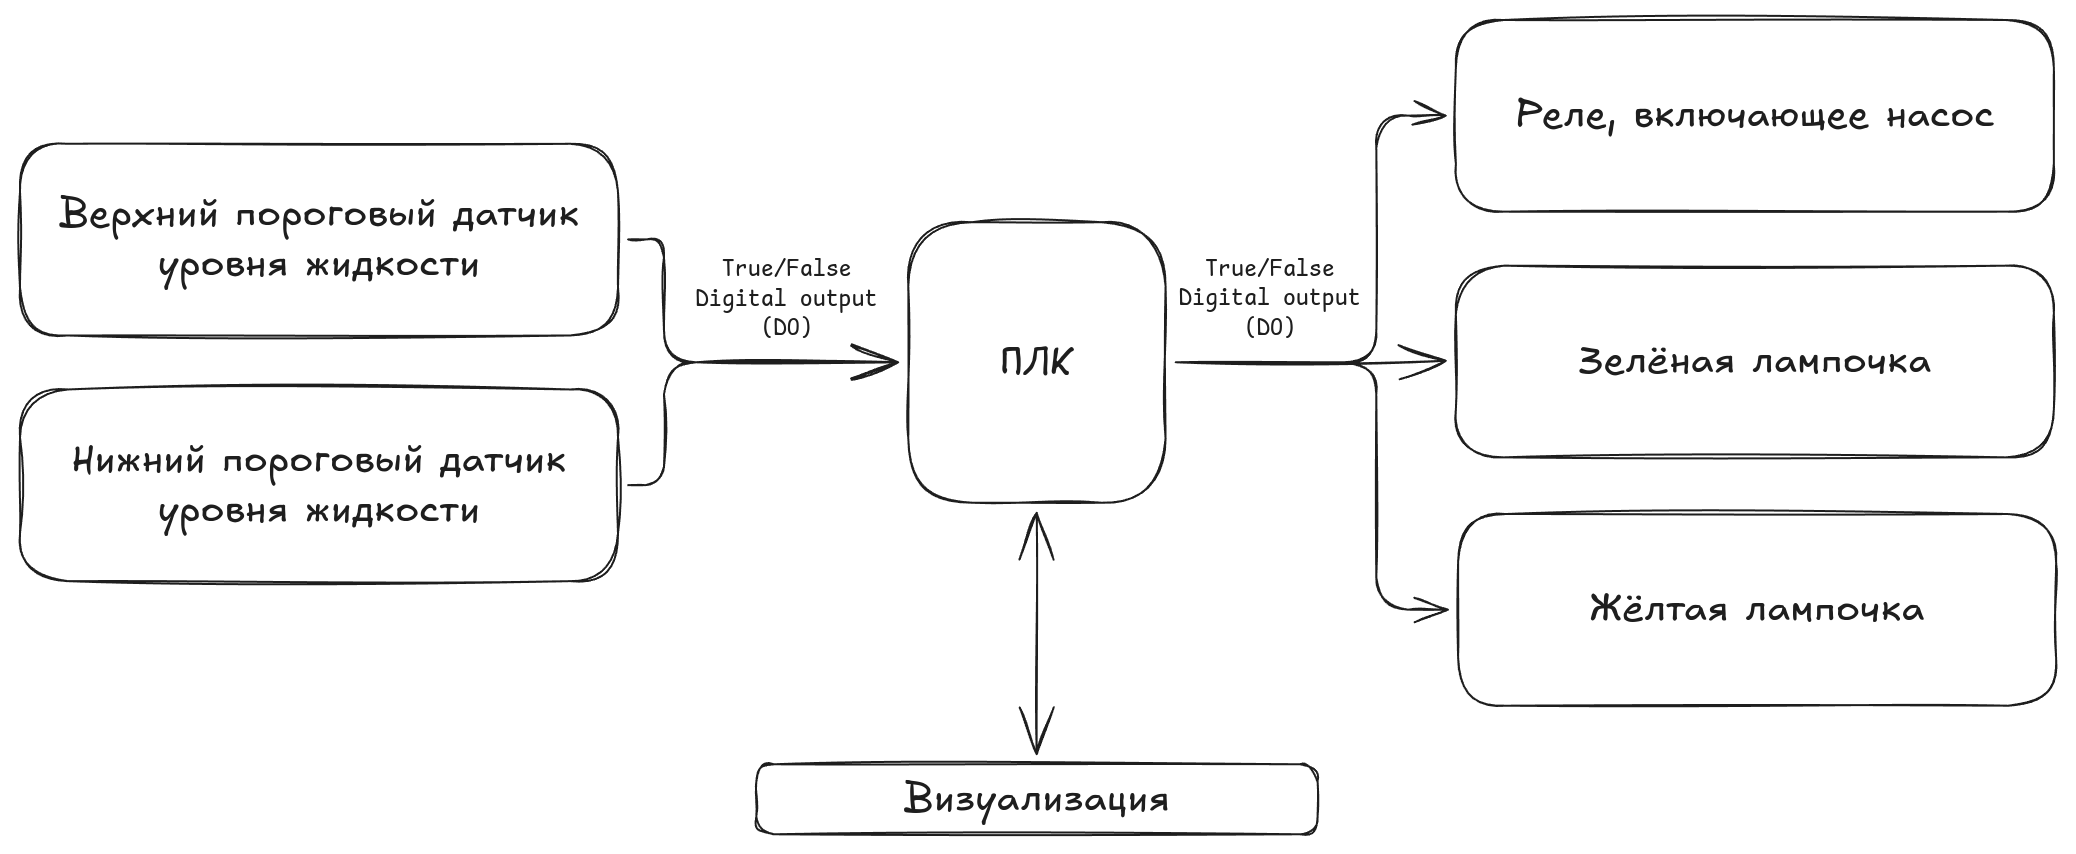
\includegraphics[width=0.71\textwidth]{sources/структурная схема.png}
\end{figure}
\addsection{Дерево задач}
\begin{figure}[H]
    \centering
    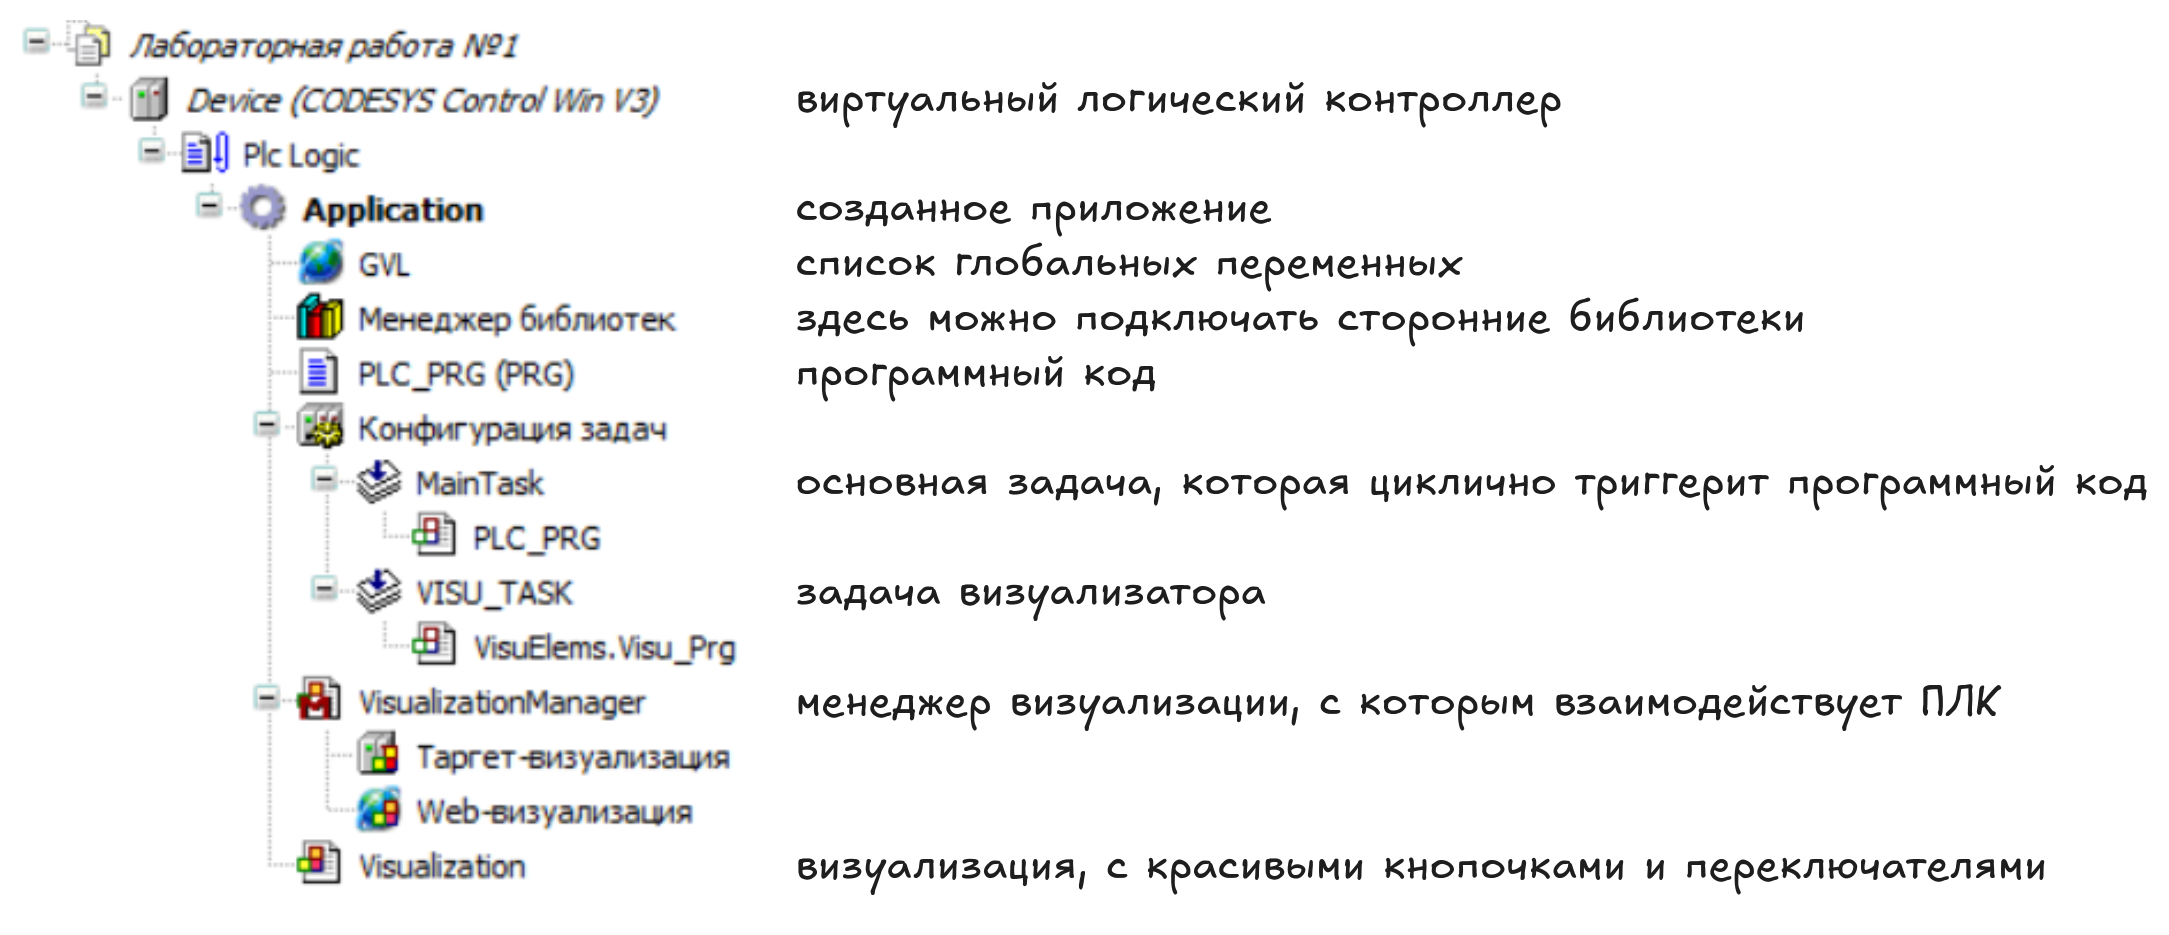
\includegraphics[width=0.66\textwidth]{sources/дерево.png}
\end{figure}
\addsection{Список глобальных переменных}
\begin{figure}[H]
    \centering
    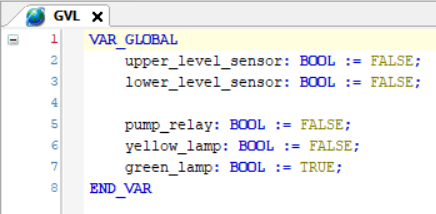
\includegraphics[width=0.33\textwidth]{sources/глобальные переменные.png}
\end{figure}
\addsection{Код программы}
\begin{lstlisting}
PROGRAM PLC_PRG
VAR
    is_pumping: BOOL := FALSE;
END_VAR

========================================

// запускать/останавливать откачку 
// только при срабатывании сенсора
IF upper_level_sensor THEN
    is_pumping := TRUE;
ELSIF lower_level_sensor THEN
    is_pumping := FALSE;
END_IF


// если откачка запущена/остановлена,
// но реле ещё не сработало/отключено,
// то включить/отключить реле и нужную лампочку
IF is_pumping AND NOT pump_relay THEN
    pump_relay := TRUE;
    yellow_lamp := TRUE;
    green_lamp := FALSE;
ELSIF NOT is_pumping AND pump_relay THEN
    pump_relay := FALSE;
    yellow_lamp := FALSE;
    green_lamp := TRUE;
END_IF
\end{lstlisting}
\addsection{Визуализация}
\begin{figure}[H]
    \centering
    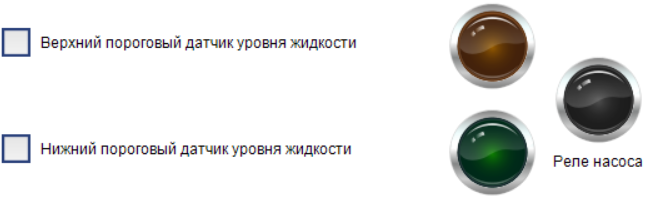
\includegraphics[width=0.6\textwidth]{sources/визуализация.png}
\end{figure}
\addsection{Демонстрация работы}
Демонстрацию работы с использованием визуализации можно посмотреть в файле \href{run:sources/демо.gif}{\texttt{sources/демо.gif}}, который располагается в папке с этим отчётом. Там же располагается и файл проекта \href{run:sources}{\texttt{Лабораторная работа №1.project}} для среды разработки Codesys 3.5.
\addsection{Заключение}
В ходе выполнения лабораторной работы была разработана программа для виртуального ПЛК Codesys Control Win V3 в системе Codesys 3.5, которая автоматизирует систему осушения подвала. Программа реализует включение насоса и лампочек при срабатывании верхнего порогового датчика уровня и выключение насоса и лампочек при срабатывании нижнего датчика уровня. Программа написана на текстовом языке ST. В результате выполнения я научился работать в среде разработки программного обеспечения для ПЛК Codesys, а также изучил основной синтаксис языка ST.
\end{document}
